

\tikzset{every picture/.style={line width=0.75pt}} %set default line width to 0.75pt        

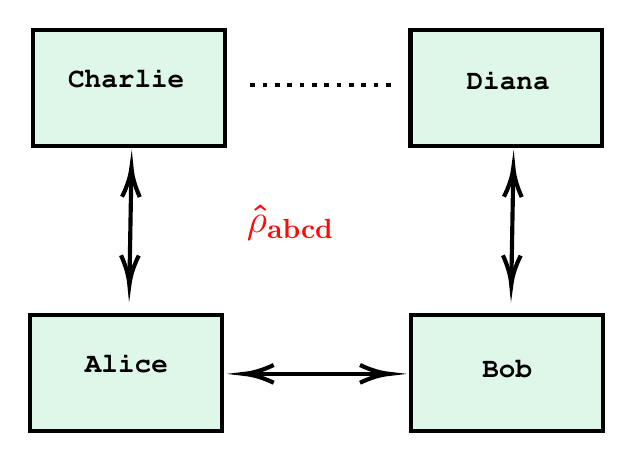
\begin{tikzpicture}[x=0.75pt,y=0.75pt,yscale=-1,xscale=1]
%uncomment if require: \path (0,300); %set diagram left start at 0, and has height of 300

%Shape: Rectangle [id:dp10277356992512154] 
\draw  [fill={rgb, 255:red, 223; green, 247; blue, 233 }  ,fill opacity=1 ][line width=1.5]  (197,162.92) -- (289.44,162.92) -- (289.44,218.97) -- (197,218.97) -- cycle ;
%Shape: Rectangle [id:dp015384298355835657] 
\draw  [color={rgb, 255:red, 0; green, 0; blue, 0 }  ,draw opacity=1 ][fill={rgb, 255:red, 223; green, 247; blue, 233 }  ,fill opacity=1 ][line width=1.5]  (198.44,25.57) -- (290.88,25.57) -- (290.88,81.63) -- (198.44,81.63) -- cycle ;
%Shape: Rectangle [id:dp7204404417404228] 
\draw  [fill={rgb, 255:red, 223; green, 247; blue, 233 }  ,fill opacity=1 ][line width=1.5]  (380.56,162.92) -- (473,162.92) -- (473,218.97) -- (380.56,218.97) -- cycle ;
%Shape: Rectangle [id:dp17140074186825027] 
\draw  [color={rgb, 255:red, 0; green, 0; blue, 0 }  ,draw opacity=1 ][fill={rgb, 255:red, 223; green, 247; blue, 233 }  ,fill opacity=1 ][line width=1.5]  (380.44,25.57) -- (472.88,25.57) -- (472.88,81.63) -- (380.44,81.63) -- cycle ;
%Straight Lines [id:da032463145441033014] 
\draw [line width=1.5]    (303.33,191.37) -- (367.32,191.37) ;
\draw [shift={(370.32,191.37)}, rotate = 180] [color={rgb, 255:red, 0; green, 0; blue, 0 }  ][line width=1.5]    (14.21,-4.28) .. controls (9.04,-1.82) and (4.3,-0.39) .. (0,0) .. controls (4.3,0.39) and (9.04,1.82) .. (14.21,4.28)   ;
\draw [shift={(300.33,191.37)}, rotate = 0] [color={rgb, 255:red, 0; green, 0; blue, 0 }  ][line width=1.5]    (14.21,-4.28) .. controls (9.04,-1.82) and (4.3,-0.39) .. (0,0) .. controls (4.3,0.39) and (9.04,1.82) .. (14.21,4.28)   ;
%Straight Lines [id:da7055775840806392] 
\draw [line width=1.5]    (245.05,145.52) -- (245.95,94.88) ;
\draw [shift={(246,91.88)}, rotate = 91.01] [color={rgb, 255:red, 0; green, 0; blue, 0 }  ][line width=1.5]    (14.21,-4.28) .. controls (9.04,-1.82) and (4.3,-0.39) .. (0,0) .. controls (4.3,0.39) and (9.04,1.82) .. (14.21,4.28)   ;
\draw [shift={(245,148.52)}, rotate = 271.01] [color={rgb, 255:red, 0; green, 0; blue, 0 }  ][line width=1.5]    (14.21,-4.28) .. controls (9.04,-1.82) and (4.3,-0.39) .. (0,0) .. controls (4.3,0.39) and (9.04,1.82) .. (14.21,4.28)   ;
%Straight Lines [id:da39607289649694266] 
\draw [color={rgb, 255:red, 0; green, 0; blue, 0 }  ,draw opacity=1 ][fill={rgb, 255:red, 44; green, 28; blue, 255 }  ,fill opacity=1 ][line width=1.5]    (429.05,145.52) -- (429.95,94.88) ;
\draw [shift={(430,91.88)}, rotate = 91.01] [color={rgb, 255:red, 0; green, 0; blue, 0 }  ,draw opacity=1 ][line width=1.5]    (14.21,-4.28) .. controls (9.04,-1.82) and (4.3,-0.39) .. (0,0) .. controls (4.3,0.39) and (9.04,1.82) .. (14.21,4.28)   ;
\draw [shift={(429,148.52)}, rotate = 271.01] [color={rgb, 255:red, 0; green, 0; blue, 0 }  ,draw opacity=1 ][line width=1.5]    (14.21,-4.28) .. controls (9.04,-1.82) and (4.3,-0.39) .. (0,0) .. controls (4.3,0.39) and (9.04,1.82) .. (14.21,4.28)   ;
%Straight Lines [id:da6546093054475423] 
\draw [line width=1.5]  [dash pattern={on 1.69pt off 2.76pt}]  (303.33,52.37) -- (332,52.37) -- (373.32,52.37) ;

% Text Node
\draw (222.06,180.54) node [anchor=north west][inner sep=0.75pt]   [align=left] {{\fontfamily{pcr}\selectfont \textbf{Alice}}};
% Text Node
\draw (213.98,43) node [anchor=north west][inner sep=0.75pt]   [align=left] {\textbf{{\fontfamily{pcr}\selectfont Charlie}}};
% Text Node
\draw (413.58,183.34) node [anchor=north west][inner sep=0.75pt]   [align=left] {\textbf{{\fontfamily{pcr}\selectfont Bob}}};
% Text Node
\draw (300.14,108.48) node [anchor=north west][inner sep=0.75pt]  [font=\Large,color={rgb, 255:red, 255; green, 8; blue, 8 }  ,opacity=1 ]  {$\mathlarger{\mathlarger{\mathlarger{\mathlarger{\mathbf{\hat{\rho }_{abcd}}}}}}$};
% Text Node
\draw (405.98,44) node [anchor=north west][inner sep=0.75pt]   [align=left] {\textbf{{\fontfamily{pcr}\selectfont Diana}}};


\end{tikzpicture}
